\documentclass[11pt]{beamer}
\usetheme{Madrid}
\usepackage[utf8]{inputenc}
\usepackage[italian]{babel}
\usepackage{amsmath}
\usepackage{amsfonts}
\usepackage{amssymb}
\usepackage{graphicx}
\usepackage{pgfplots}
\usetikzlibrary{patterns}
\graphicspath{ {./media/} }
\pgfplotsset{width=9.5cm,compat=1.18}

\author[Barbaro, Bifulco, Sansonetti]{\small Nicola Barbaro (1070668)\linebreak Mario Bifulco (881727)\linebreak Franco Sansonetti (1087075)}
\title{Sliding Block Puzzle - Sviluppo in PROLOG}
\setbeamertemplate{navigation symbols}{}
\date{A.A. 2022/2023}
\institute[]{Università degli studi di Torino\\Intelligenza Artificiale e Laboratorio}  

\begin{document}

\begin{frame}
\titlepage
\end{frame}

\begin{frame}
\frametitle{Il gioco, le regole}
\begin{itemize}
    \item La board
    \item In cosa consiste il gioco
    \item Come eseguire una mossa sulla board
\end{itemize}
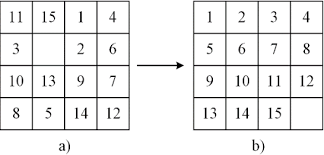
\includegraphics[scale=0.8]{scrambledtosolved.png}
\centering
\end{frame}

\begin{frame}
\frametitle{Il problema come ricerca nello spazio degli stati}
\begin{itemize}
    \item Rappresentazione del problema come albero $T  = (N, A)$
    \item Per ogni mossa possibile, un possibile sottoalbero radicato in quella nuova posizione
    \item Strategie di traversazione dell'albero valutate e testate  (\emph{ID}, \emph{IDA*})
    \item Focus sulla efficienza computazionale nel progetto
\end{itemize}
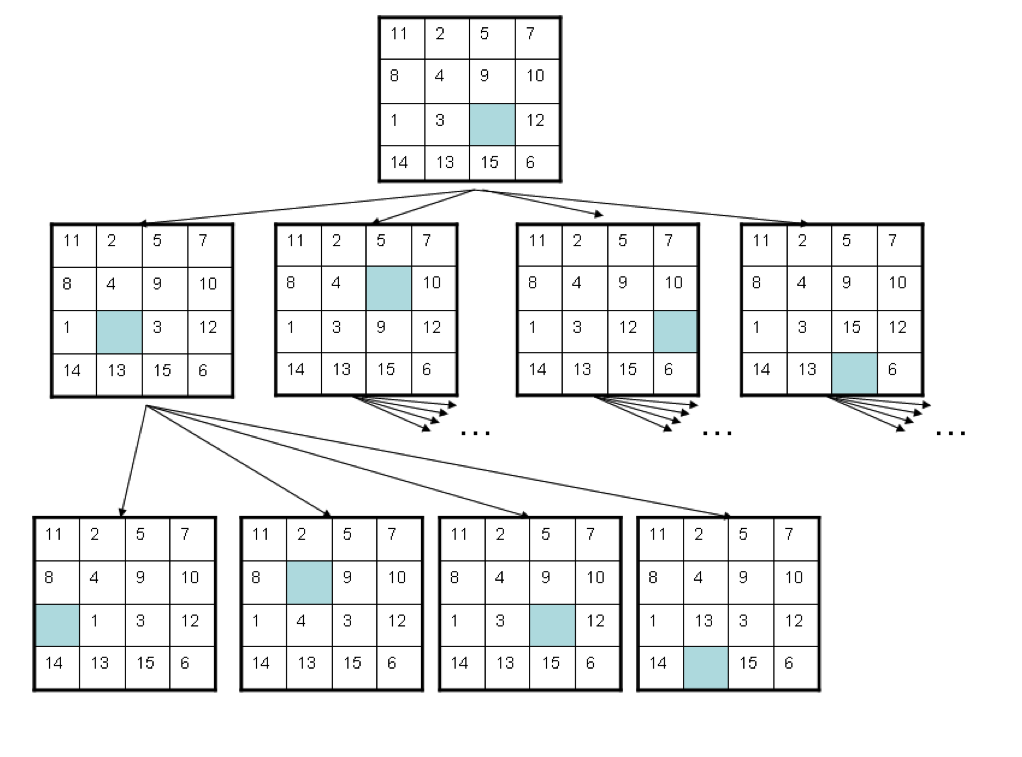
\includegraphics[scale=0.4]{tree.png}
\centering
\end{frame}


\begin{frame}
    \frametitle{Le posizioni in memoria}
    \begin{enumerate}
        \item \begin{table}
            \begin{tabular}{|c|c|c|c|}
                \hline
                2 & 4 & 1 & 3 \\ \hline
                14 & 12 &  & 8  \\  \hline
                7 & 5 & 13 & 15 \\ \hline
                11 & 6 & 10 & 9 \\ \hline
            \end{tabular}
        \end{table}
        \item 2,4,1,3,14,12,v,8,7,5,13,15,11,6,10,9
        \item la posizione viene parsata attraverso hashing esadecimale: $0x20401030e0c100807050d0f0b060a09$
        \item conversione in intero decimale: $2679245703445435204062882741413612041$
    \end{enumerate}
    Viene registrato un risparmio in memoria di svariati ordini: in genere, a profondità $\geq 15$, da oltre 6GB a pochi MB.
\end{frame}


\begin{frame}
    \frametitle{Le mosse (con un esempio: la mossa U - Parte 1)}
    a partire dalla posizione $pos = 0x204{\color{blue}01}030e0c{\color{red}10}0807050d0f0b060a09$
    \begin{enumerate}
    \item Sapendo che la posizione della cella blank è {\color{red} $9$}, la cella di arrivo dopo la mossa U è in posizione {\color{blue} $9+4 = 13$}
    \item La cifra che si trova in posizione {\color{blue} 13} non è nota a priori, dato che conserviamo un singolo intero e non una lista, va estratto:
        \begin{itemize}
    	\item dato un numero binario $bucket = bin(15 << 8*{\color{blue} 13})$
    	\item l'algoritmo estrae $swap = (pos\&bucket) >> 8*{\color{blue} 13} = {\color{blue} 1}$, che è effettivamente il valore in Up rispetto al blank
    	\end{itemize}
    \end{enumerate}
\end{frame}

\begin{frame}
    \frametitle{Le mosse (con un esempio: la mossa U - Parte 2)}
    a partire dalla posizione $pos = 0x204{\color{blue}01}030e0c{\color{red}10}0807050d0f0b060a09$
    \begin{enumerate}
        \setcounter{enumi}{4}
    \item calcoliamo $diff  = blank - swap = 16 - 1 = {\color{green}15}$, la differenza tra il valore di blank (rappresentato come 16) e il valore da swappare
    \item Con una strategia del tutto analoga all'accesso alla cella di destinazione, accediamo nuovamente alla posizione {\color{blue}13} per \emph{aggiungere} il valore della variable $diff$, trasformando 1 in 16 (1+15)
    \item Ancora, accediamo alla posizione {\color{blue}9} per \emph{sottrarre} il valore della variable $diff$, trasformando 16 in 1 (16-15)
    \item le altre celle restano invariate.
    \end{enumerate}
    risulta: $new\_pos = 0x204{\color{blue}10}030e0c{\color{red}01}0807050d0f0b060a09$
\end{frame}


\begin{frame}
\frametitle{Le Euristiche}
\begin{itemize}
    \item È una funzione $h(n)$, che stima il costo minimo da ogni vertice $n$ del grafo al goal.
    \item Ammissibilità: $g(n) \geq h(n)$, ossia non sovrastima mai il reale costo per raggiungere un goal.
    \item Consistenza: $c(n, n') + h(n') \geq h(n)$, ossia non sovrastima mai il costo verso un successore $n'$ di $n$ sommato a $h(n')$  
\end{itemize}
\centering
\end{frame}

\begin{frame}
\frametitle{Le Euristiche: La Distanza Di Manhattan}
\begin{itemize}
    \item Somma delle distanze di ogni singola cella sulla board rispetto alla sua posizione originaria 
    \item Sia Ammissibile che Consistente
    \item L'efficienza risulta importante: Da $O(n^2)$ a $O(1)$
    \item Facile da Rilassare: overhead permette di risolvere anche le posizioni più complesse in pochi secondi, a discapito dell'ammissibilità
\end{itemize}
\centering
\end{frame}


\begin{frame}
\frametitle{Le Euristiche: I Conflitti Lineari}
\begin{itemize}
    \item Due tiles sono in conflitto lineare se sono sulla riga/colonna corretta ma vanno swappate
    \item Sia Ammissibile che Consistente
    \item Complessità $O(n^2)$, necessario uno sviluppo ottimizzato 
    \item Essendo un caso specifico, molto spesso l'euristica aggiunge un overhead di complessità senza ottenere benefici
\end{itemize}
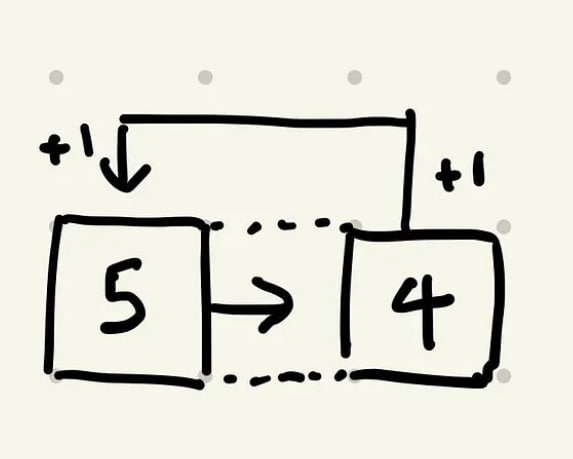
\includegraphics[scale=0.25]{linearconflict.jpg}
\centering
\end{frame}

\begin{frame}
\frametitle{Risultati}
\begin{tikzpicture}[yscale=4]
    \draw (-1.5,0)--(3,0) (-1,0)--(-1,.75);
    \draw[pattern=north east lines] (-.5,0) rectangle (.5,.25) (.5,0) rectangle (1.5,.5) (1.5,0) rectangle (2.5,.25);
    \foreach \x in {ID, MD, MD + LC} 
     \draw (\x,0) -- (\x,-1pt) node[below]{\footnotesize\x};
    \foreach \y in {0.25,0.50} 
     \draw (-1,\y) -- ({-1cm-4pt},\y) node[left]{\footnotesize\y};
    \end{tikzpicture}
\end{frame}

\end{document}